%
% ---------------------------------------------------------------
% Copyright (C) 2012-2018 Gang Li
% ---------------------------------------------------------------
%
% This work is the default powerdot-tuliplab style test file and may be
% distributed and/or modified under the conditions of the LaTeX Project Public
% License, either version 1.3 of this license or (at your option) any later
% version. The latest version of this license is in
% http://www.latex-project.org/lppl.txt and version 1.3 or later is part of all
% distributions of LaTeX version 2003/12/01 or later.
%
% This work has the LPPL maintenance status "maintained".
%
% This Current Maintainer of this work is Gang Li.
%
%

\documentclass[
 size=14pt,
 paper=smartboard,  %a4paper, smartboard, screen
 mode=present, 		%present, handout, print
 display=slides, 	% slidesnotes, notes, slides
 style=tuliplab,  	% TULIP Lab style
 pauseslide,
 fleqn,leqno]{powerdot}
\thispagestyle{empty}

\usepackage{cancel}
\usepackage{caption}
\usepackage{stackengine}
\usepackage{smartdiagram}
\usepackage{attrib}
\usepackage{amssymb}
\usepackage{amsmath} 
\usepackage{amsthm} 
\usepackage{mathtools}
\usepackage{rotating}
\usepackage{graphicx}
\usepackage{boxedminipage}
\usepackage{rotate}
\usepackage{calc}
\usepackage[absolute]{textpos}
\usepackage{psfrag,overpic}
\usepackage{fouriernc}
\usepackage{pstricks,pst-3d,pst-grad,pstricks-add,pst-text,pst-node,pst-tree}
\usepackage{moreverb,epsfig,subfigure}
\usepackage{color}
\usepackage{booktabs}
\usepackage{etex}
\usepackage{breqn}
\usepackage{multirow}
\usepackage{natbib}
\usepackage{bibentry}
\usepackage{gitinfo2}
\usepackage{siunitx}
\usepackage{nicefrac}
%\usepackage{geometry}
%\geometry{verbose,letterpaper}
\usepackage{media9}
\usepackage{animate}
%\usepackage{movie15}
\usepackage{auto-pst-pdf}

\usepackage{breakurl}
\usepackage{fontawesome}
\usepackage{xcolor}
\usepackage{multicol}



\usepackage{verbatim}
\usepackage[utf8]{inputenc}
\usepackage{/usr/local/texlive/dtk-logos}
\usepackage{tikz}
\usepackage{adigraph}
%\usepackage{tkz-graph}
\usepackage{hyperref}
%\usepackage{ulem}
\usepackage{pgfplots}
\usepackage{verbatim}
\usepackage{fontawesome}


\usepackage{todonotes}
% \usepackage{pst-rel-points}
\usepackage{animate}
\usepackage{fontawesome}

\usepackage{listings}
\lstset{frameround=fttt,
frame=trBL,
stringstyle=\ttfamily,
backgroundcolor=\color{yellow!20},
basicstyle=\footnotesize\ttfamily}
\lstnewenvironment{code}{
\lstset{frame=single,escapeinside=`',
backgroundcolor=\color{yellow!20},
basicstyle=\footnotesize\ttfamily}
}{}


\usepackage{hyperref}
\hypersetup{ % TODO: PDF meta Data
  pdftitle={Presentation Title},
  pdfauthor={Gang Li},
  pdfpagemode={FullScreen},
  pdfborder={0 0 0}
}


% \usepackage{auto-pst-pdf}
% package to show source code

\definecolor{LightGray}{rgb}{0.9,0.9,0.9}
\newlength{\pixel}\setlength\pixel{0.000714285714\slidewidth}
\setlength{\TPHorizModule}{\slidewidth}
\setlength{\TPVertModule}{\slideheight}
\newcommand\highlight[1]{\fbox{#1}}
\newcommand\icite[1]{{\footnotesize [#1]}}

\newcommand\twotonebox[2]{\fcolorbox{pdcolor2}{pdcolor2}
{#1\vphantom{#2}}\fcolorbox{pdcolor2}{white}{#2\vphantom{#1}}}
\newcommand\twotoneboxo[2]{\fcolorbox{pdcolor2}{pdcolor2}
{#1}\fcolorbox{pdcolor2}{white}{#2}}
\newcommand\vpspace[1]{\vphantom{\vspace{#1}}}
\newcommand\hpspace[1]{\hphantom{\hspace{#1}}}
\newcommand\COMMENT[1]{}

\newcommand\placepos[3]{\hbox to\z@{\kern#1
        \raisebox{-#2}[\z@][\z@]{#3}\hss}\ignorespaces}

\renewcommand{\baselinestretch}{1.2}


\newcommand{\draftnote}[3]{
	\todo[author=#2,color=#1!30,size=\footnotesize]{\textsf{#3}}	}
% TODO: add yourself here:
%
\newcommand{\gangli}[1]{\draftnote{blue}{GLi:}{#1}}
\newcommand{\shaoni}[1]{\draftnote{green}{sn:}{#1}}
\newcommand{\gliMarker}
	{\todo[author=GLi,size=\tiny,inline,color=blue!40]
	{Gang Li has worked up to here.}}
\newcommand{\snMarker}
	{\todo[author=Sn,size=\tiny,inline,color=green!40]
	{Shaoni has worked up to here.}}


%\input{../../../.git/gitHeadInfo.gin}

%%%%%%%%%%%%%%%%%%%%%%%%%%%%%%%%%%%%%%%%%%%%%%%%%%%%%%%%%%%%%%%%%%%%
% title
% TODO: Customize to your Own Title, Name, Address
%

\title{Sales of Books Forecasting}
\author{
Lin Jiahong
\\
\\Nanjing University of Science and Technology
}
\date{\gitCommitterDate}


% Customize the setting of slides
\pdsetup{
% TODO: Customize the left footer, and right footer
rf=\href{http://www.tulip.org.au}{
Last Changed by: \textsc{\gitCommitterName}\ \gitVtagn-\gitAbbrevHash\ (\gitAuthorDate)
},
cf={Sales of Books Forecasting},
}
\begin{document}

\maketitle

%\begin{slide}{Overview}
%\tableofcontents[content=sections]
%\end{slide}


%%==========================================================================================
%%
\begin{slide}[toc=,bm=]{Overview}
\tableofcontents[content=currentsection,type=1]
\end{slide}
%%
%%==========================================================================================


\section{Problem Definition}


%%==========================================================================================
%%
\begin{slide}{Sales of Books Forecast}
\begin{center}
\twotonebox{\rotatebox{90}{Defn}}{\parbox{.86\textwidth}
{Sales of Books Forecast aims to predict the sales of books in 2021 through the book sales data from 2017 to 2020. 
\begin{itemize}
\item Data covers different  \textcolor{orange}{countries} 
and different \textcolor{orange}{stores}.
\item There are cyclical and seasonal changes in book sales.
\end{itemize}
}}

\end{center}
\begin{center}
	\begin{tabular}{c| c c c c c }
		\toprule
		%\centering
		Data & \texttt{row_num}  & \texttt{date} & \texttt{country} & \texttt{store} & \texttt{product }\\
		\midrule
		$train$
		&  {$70128$} &  {$1461$} &  {$6$} &  {$2$}&  {$4$} \\
		$test$
		&  {$17520$} &  {$365$} &  {$6$} &  {$2$}&  {$4$} \\
		\bottomrule
	\end{tabular}
\end{center}
%%============================================================================

\end{slide}
%%
%%==========================================================================================






\section{Data Analysis}





%%==========================================================================================
%%
\begin{slide}[toc=,bm=]{Overall data}

\begin{itemize}
\item
Country - \textcolor{orange} {Belgium,France,Germany,Italy,Poland,Spain}
\end{itemize}

\begin{itemize}
	\item
	Product - \textcolor{orange} {[Kaggle Advanced Techniques],[Kaggle Getting Started],[Kaggle Recipe Book],[Kaggle for Kids: One Smart Goose]}
\end{itemize}

\begin{itemize}
	\item
	Stores - \textcolor{orange} {KaggleMart,KaggleRama}
\end{itemize}

\begin{itemize}
	\item
	Time line
\end{itemize}

\begin{center}
	\begin{tabular}{c| c |c }
		\toprule
		%\centering
		Data & \texttt{Earliest date}  & \texttt{Latest date} \\
		\midrule
		$train$
		&  {$2017-01-01$} &  {$2020-12-31$} \\
		$test$
		&  {$2021-01-01$} &  {$2021-12-31$}  \\
		\bottomrule
	\end{tabular}
\end{center}
%%==========================================================================================


\end{slide}
%%
%%==========================================================================================


%%==========================================================================================
%%
\begin{slide}[toc=,bm=]{Monthly sales statistics}
\begin{itemize}
	\item
	the patterns in sales of all countries and stores are identical.the magnitudes of sales are different
\end{itemize}
\begin{figure}
  \centering
  \selectcolormodel{rgb}
  \includegraphics[scale=0.23]{month.eps}
%  \includegraphics[width=0.5\textwidth]{figures//OutAspect_target.eps}\\
  \caption{Monthly sales}\label{fig:OutAspect-target}
\end{figure}
\end{slide}
%%
%%==========================================================================================


==============
%%
\begin{slide}[toc=,bm=]{Aggregating Time Series(Store)}
	
\begin{itemize}
	\bigskip
	\item
 	Store-KaggleMart appears to consistantly have ~74.25\% of the total number of sales
\end{itemize}
\bigskip
\begin{center}
\twocolumn{
	\begin{center}
\begin{tabular}{c| c }
	\toprule
	%\centering
	Store & \texttt{ratio}  \\
	\midrule
	$KaggleMart$
	&  {$0.742515$}  \\
	$KaggleRama$
	&  {$0.257485$}  \\
	\bottomrule
\end{tabular}
\end{center}
}{
\begin{center}
\begin{figure}
	\centering
	\selectcolormodel{rgb}
	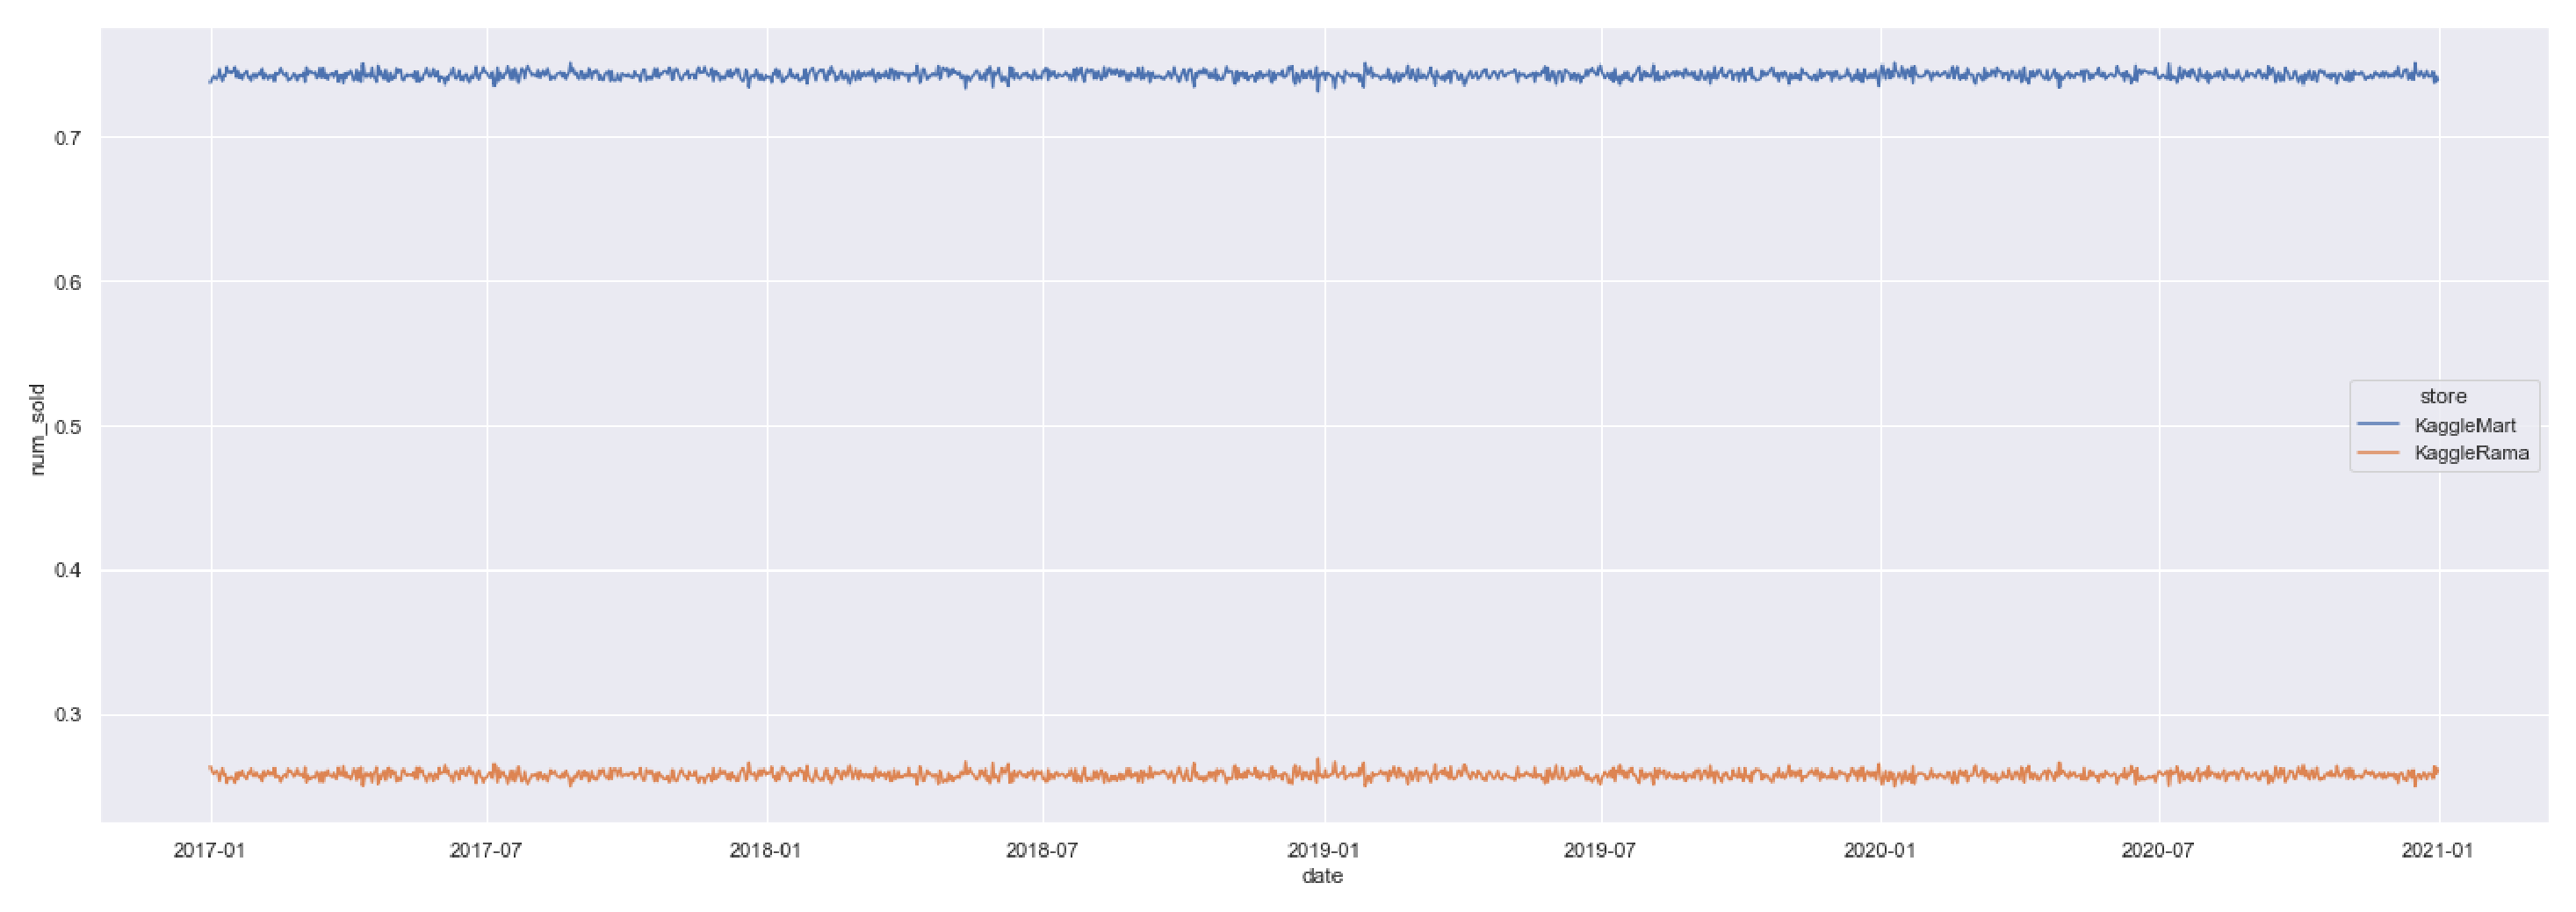
\includegraphics[scale=0.21]{store-ratio.eps}
	%  \includegraphics[width=0.5\textwidth]{figures//OutAspect_target.eps}\\
	\caption{Stores ratio}\label{fig:OutAspect-target}
\end{figure}
\end{center}
}
\end{center}
\end{slide}
%%
%%==========================================================================================

==============
%%
\begin{slide}[toc=,bm=]{Aggregating Time Series(Store)}
	\begin{itemize}
		\item
		To compare the trend of the two stores, multiply the sales data of the two stores by a constant.
	\end{itemize}
			\begin{figure}
				\centering
				\selectcolormodel{rgb}
				\includegraphics[scale=0.225]{store-trend.eps}
				%  \includegraphics[width=0.5\textwidth]{figures//OutAspect_target.eps}\\
				\caption{Stores ratio trend}\label{fig:OutAspect-target}
			\end{figure}
\end{slide}
%%
%%==========================================================================================

==============
%%
\begin{slide}[toc=,bm=]{Aggregating Time Series(Country)}
	
	\begin{itemize}
		\bigskip
		\item
		Country-The ratio of total sales in different countries also fluctuates little.
	\end{itemize}
	\bigskip
	\begin{center}
		\twocolumn{
			\begin{center}
			\begin{tabular}{c| c }
				\toprule
				%\centering
				Country & \texttt{ratio}  \\
				\midrule
				$Belgium$
				&  {$0.218930$}  \\
				$France$
				&  {$0.191360$}  \\
				$Germany $
				&  {$0.219586$}  \\
				$Italy$
				&  {$0.159383$}  \\
				$Poland$
				&  {$0.071348$}  \\
				$Spain$
				&  {$0.139393$}  \\
				\bottomrule
			\end{tabular}
			\end{center}
		}{
			\begin{figure}
				\centering
				\selectcolormodel{rgb}
				\includegraphics[scale=0.215]{Country-ratio.eps}
				%  \includegraphics[width=0.5\textwidth]{figures//OutAspect_target.eps}\\
				\caption{Countries ratio}\label{fig:OutAspect-target}
			\end{figure}
		}
	\end{center}
\end{slide}
%%
%%==========================================================================================

==============
%%
\begin{slide}[toc=,bm=]{Aggregating Time Series(Country)}
	\begin{itemize}
		\item
		Multiply all countries by a constant so they are comparable with Belgium.
	\end{itemize}
		\begin{figure}
			\centering
			\selectcolormodel{rgb}
			\includegraphics[scale=0.235]{Country-trend.eps}
			%  \includegraphics[width=0.5\textwidth]{figures//OutAspect_target.eps}\\
			\caption{Countries ratio trend}\label{fig:OutAspect-target}
		\end{figure}

\end{slide}
%%
%%==========================================================================================

==============
%%
\begin{slide}[toc=,bm=]{Aggregating Time Series(Country and Store)}
	\begin{itemize}
		\item
		In the plots make all time series inline with the Belgium KaggleMart store by multiplying by a constant.
	\end{itemize}
		\begin{figure}
			\centering
			\selectcolormodel{rgb}
			\includegraphics[scale=0.23]{Countryandstore-trend.eps}
			%  \includegraphics[width=0.5\textwidth]{figures//OutAspect_target.eps}\\
			\caption{Countries and Store trend}\label{fig:OutAspect-target}
		\end{figure}
\end{slide}
%%
%%==========================================================================================

==============
%%
\begin{slide}[toc=,bm=]{Aggregating Time Series(Product)}
	\begin{itemize}
		\item
		The change trend of the sales volume of the four books is cyclical.
	\end{itemize}

		\begin{figure}
			\centering
			\selectcolormodel{rgb}
			\includegraphics[scale=0.4]{product.eps}
			%  \includegraphics[width=0.5\textwidth]{figures//OutAspect_target.eps}\\
			\caption{Sales of Product}\label{fig:OutAspect-target}
		\end{figure}

\end{slide}
%%
%%==========================================================================================

==============
%%
\begin{slide}[toc=,bm=]{Aggregating Time Series(Product)}
	\begin{itemize}
		\item
		The change trend of the sales proportion of the four books has rules.
	\end{itemize}
		\begin{figure}
			\centering
			\selectcolormodel{rgb}
			\includegraphics[scale=0.4]{product-trend.eps}
			%  \includegraphics[width=0.5\textwidth]{figures//OutAspect_target.eps}\\
			\caption{Product ratio trend}\label{fig:OutAspect-target}
		\end{figure}
\end{slide}
%%
%%==========================================================================================

==============
%%
\begin{slide}[toc=,bm=]{Aggregated Time Series}
	\begin{itemize}
		\item
		aggregate the sales timeline to consider how to forecast the overall sales volume.
	\end{itemize}
	\begin{figure}
		\centering
		\selectcolormodel{rgb}
		\includegraphics[scale=0.4]{trainline.eps}
		%  \includegraphics[width=0.5\textwidth]{figures//OutAspect_target.eps}\\
		\caption{Aggregated time series}\label{fig:OutAspect-target}
	\end{figure}
\end{slide}
%%
%%==========================================================================================
\section{Feature Extraction}


\begin{slide}[toc=,bm=]{Forecast target}
	\begin{itemize}
		\item
		the total sales of each day.
		\item
		the sales volume of different products in each day of the year.
	\end{itemize}
	\begin{figure}
		\centering
		\selectcolormodel{rgb}
		\includegraphics[scale=0.4]{trainline.eps}
		%  \includegraphics[width=0.5\textwidth]{figures//OutAspect_target.eps}\\
		\caption{Aggregated time series}\label{fig:OutAspect-target}
	\end{figure}
\end{slide}
%%
%%==========================================================================================


%%==========================================================================================
%%
\begin{slide}[toc=,bm=]{Time Feature Extraction}
		\begin{itemize}
		\item
Seasonal patterns in sales were discovered through ob-
servation. We extracted features such as the month of the year, the day of the week, and the day of the year from the time series.
\end{itemize}

	\begin{figure}
		\centering
		\selectcolormodel{rgb}
		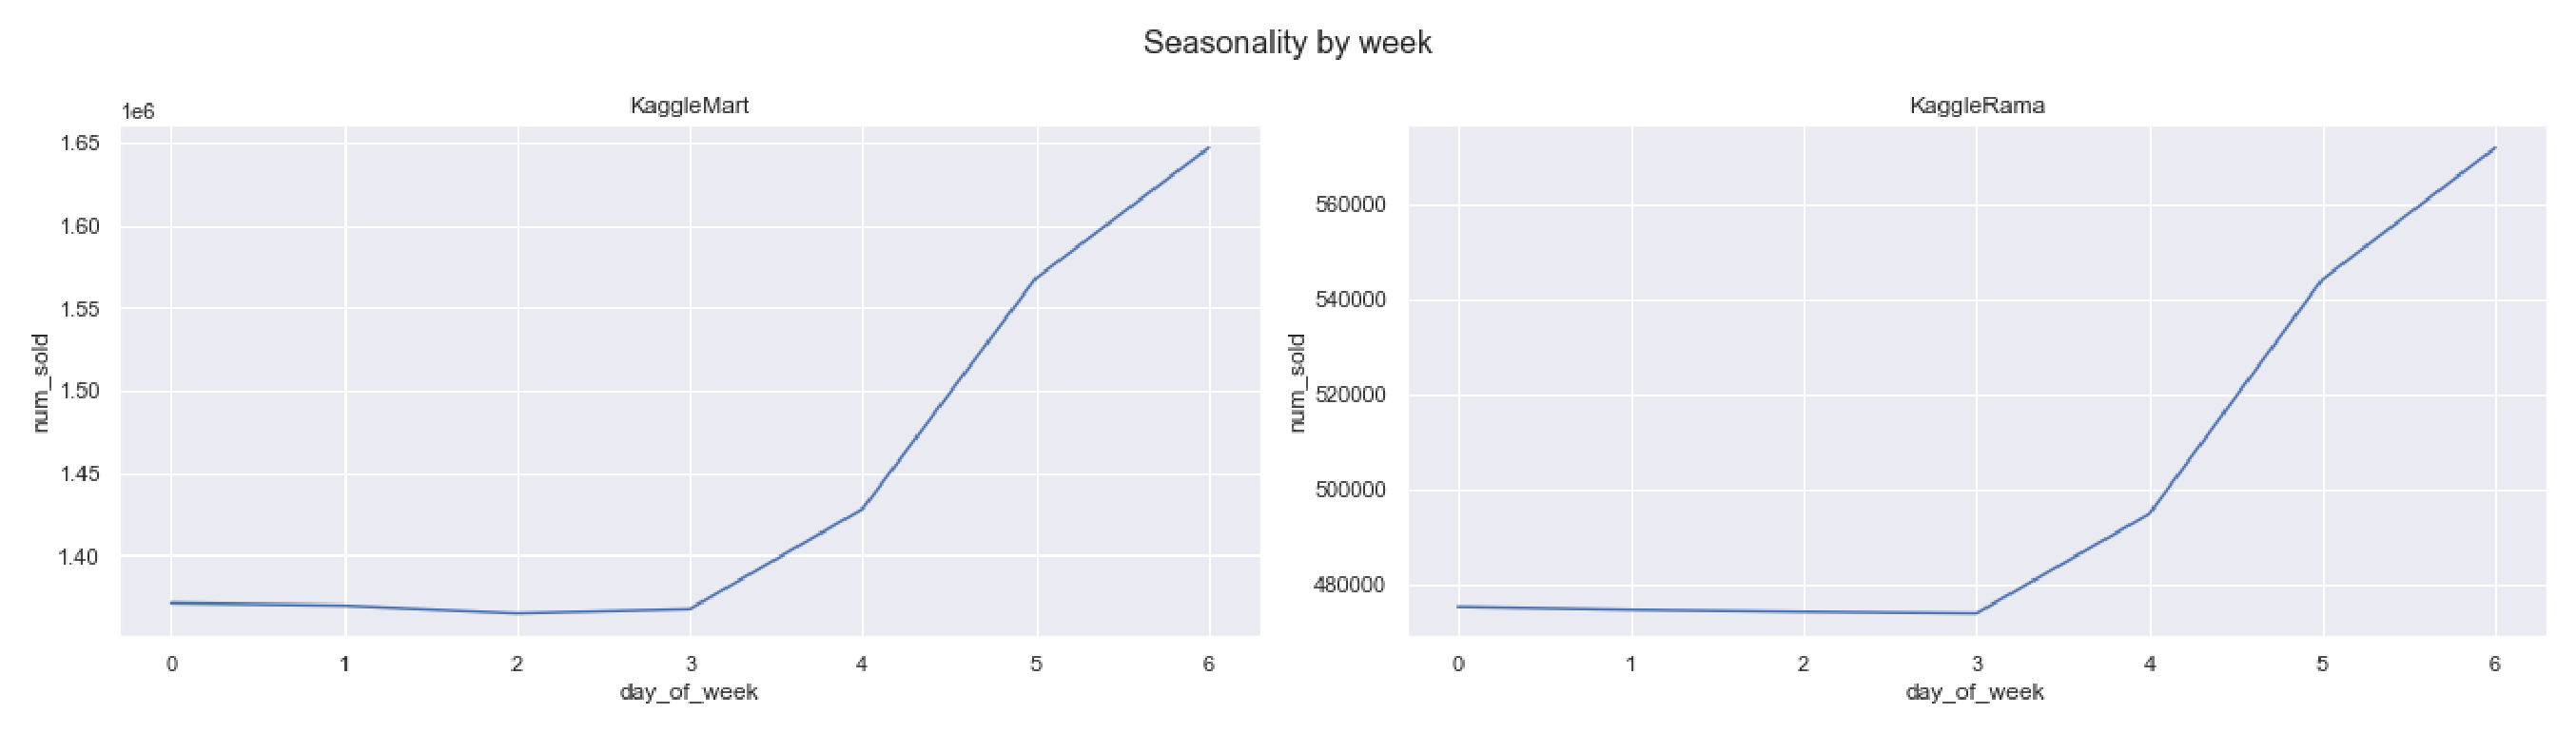
\includegraphics[scale=0.4]{week-feature.eps}
		%  \includegraphics[width=0.5\textwidth]{figures//OutAspect_target.eps}\\
		\caption{weekday feature}\label{fig:OutAspect-target}
	\end{figure}
\end{slide}
%%
%%==========================================================================================


%%==========================================================================================
%%
\begin{slide}[toc=,bm=]{Time Feature Extraction}
		\begin{itemize}
	\item
We converted the monthly data into numerical values that are suitable for input
into a Fourier transform. This allows us to perform a Fourier transform on the monthly data and obtain the coefficients of the various frequency components.
	\item
	Also took into account features related to important dates within the year.
	\item
	The features of the training set include \textcolor{orange} {23}  feature items.
	\end{itemize}
	\begin{center}
	\begin{tabular}{c| c }
		\toprule
		%\centering
		feature & \texttt{value}  \\
		\midrule
		$month\_sin$
		&  {$0.5$}  \\
		$month\_cos$
		&  {$0.866025$}  \\
		$year$
		&  {$2020$}  \\
		$important\_dates\_1$
		&  {$0/1$}  \\
		$day\_of\_week\_1$
		&  {$0/1$}  \\
		\bottomrule
	\end{tabular}
\end{center}
%	\begin{figure}
%		\centering
%		\selectcolormodel{rgb}
%		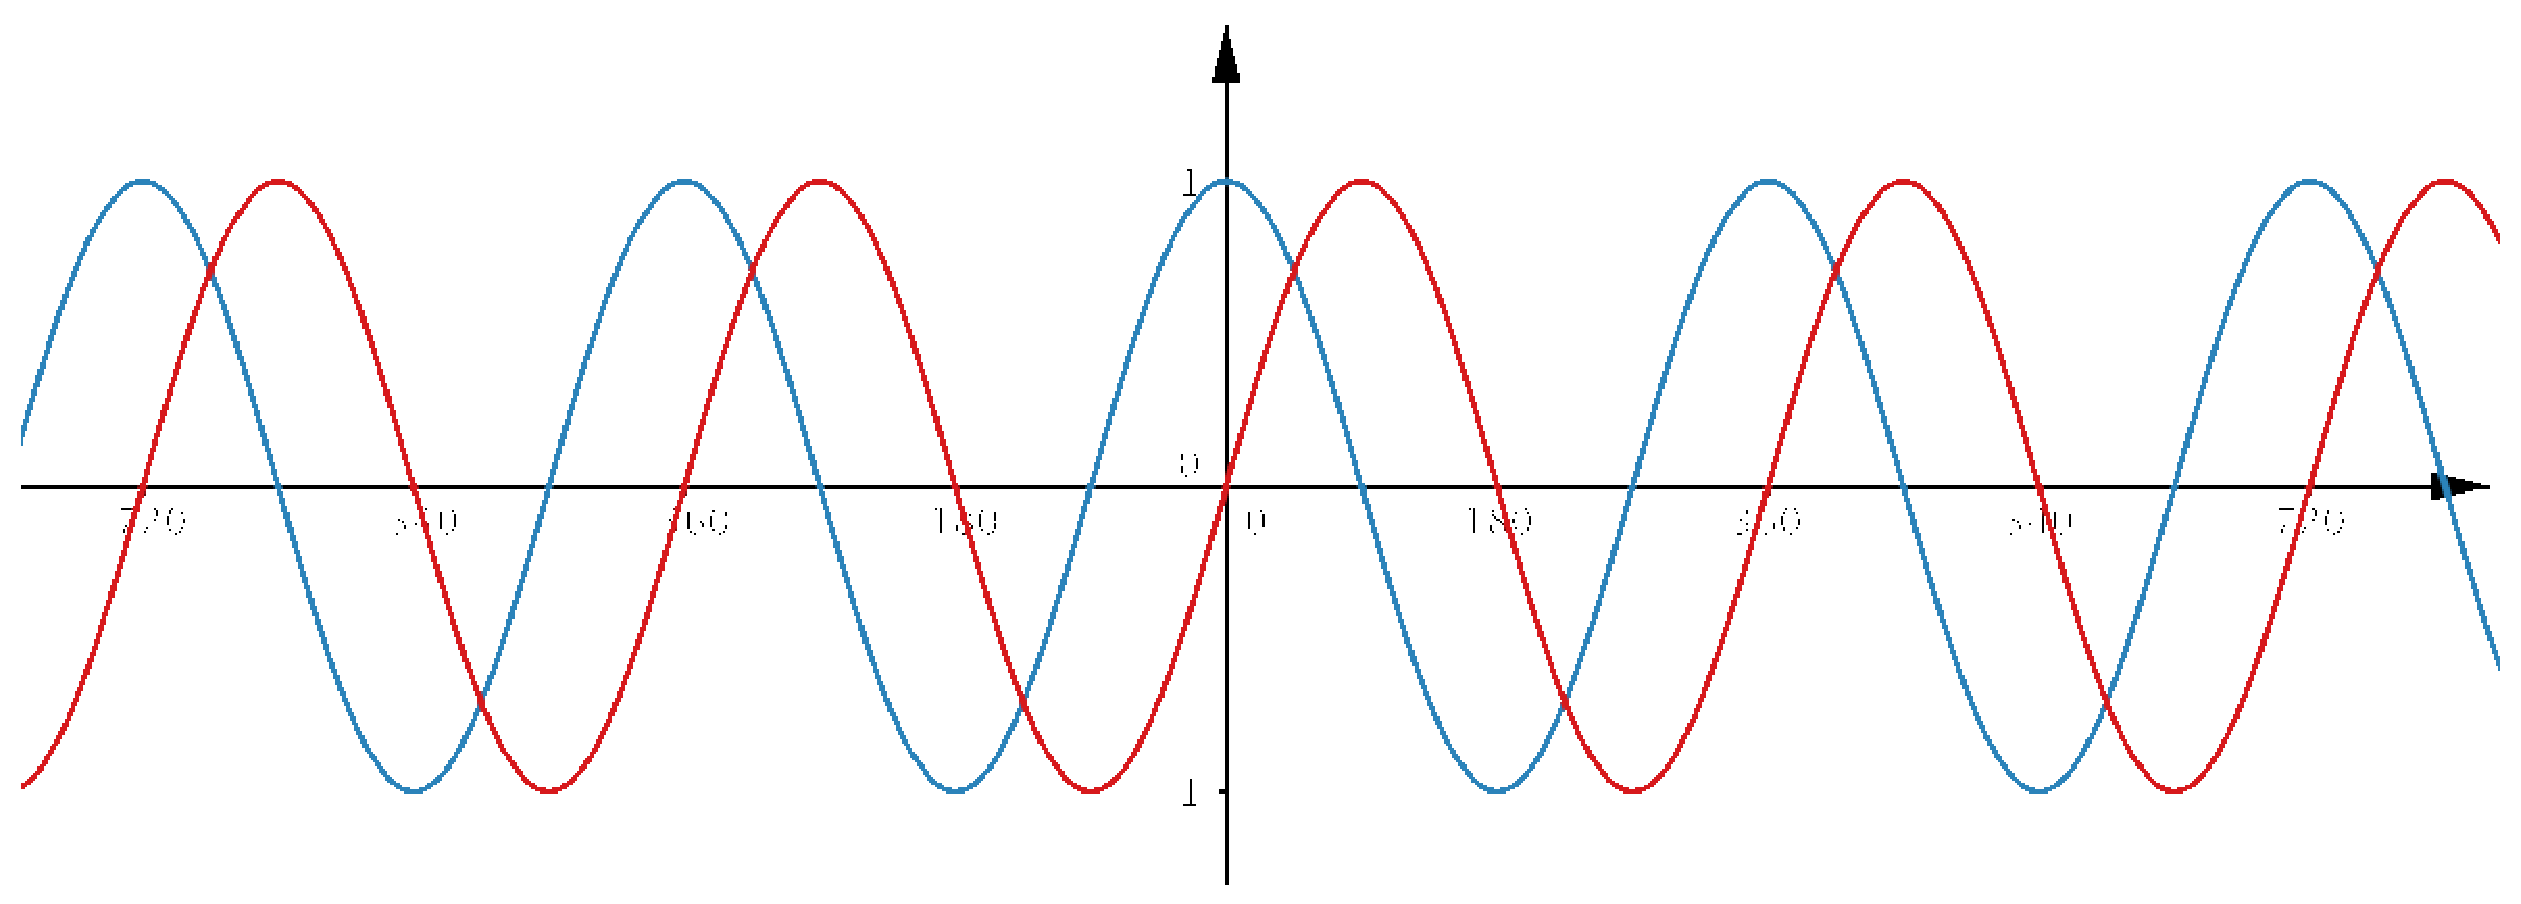
\includegraphics[scale=0.4]{fourier.eps}
%		%  \includegraphics[width=0.5\textwidth]{figures//OutAspect_target.eps}\\
%		\caption{weekday feature}\label{fig:OutAspect-target}
%	\end{figure}



\end{slide}
%%
%%==========================================================================================


\section{Model Train}


%%==========================================================================================
%%
\begin{slide}[toc=,bm=]{Total Sales Forecasting}
		\begin{itemize}
	\item
	Use Ridge regression from the  \textcolor{orange}{"linear\_model"} module to correlate the relationship between\textcolor{orange}{sales}  and \textcolor{orange}{time features} , and predict on the test set.
	\item
	Train the model with time features as \textcolor{orange}{X} and sales as \textcolor{orange}{y}. 
		\item 
		The sales of the test set is predicted according to the time features of the test set.
\end{itemize}
	\begin{figure}
	\centering
	\selectcolormodel{rgb}
	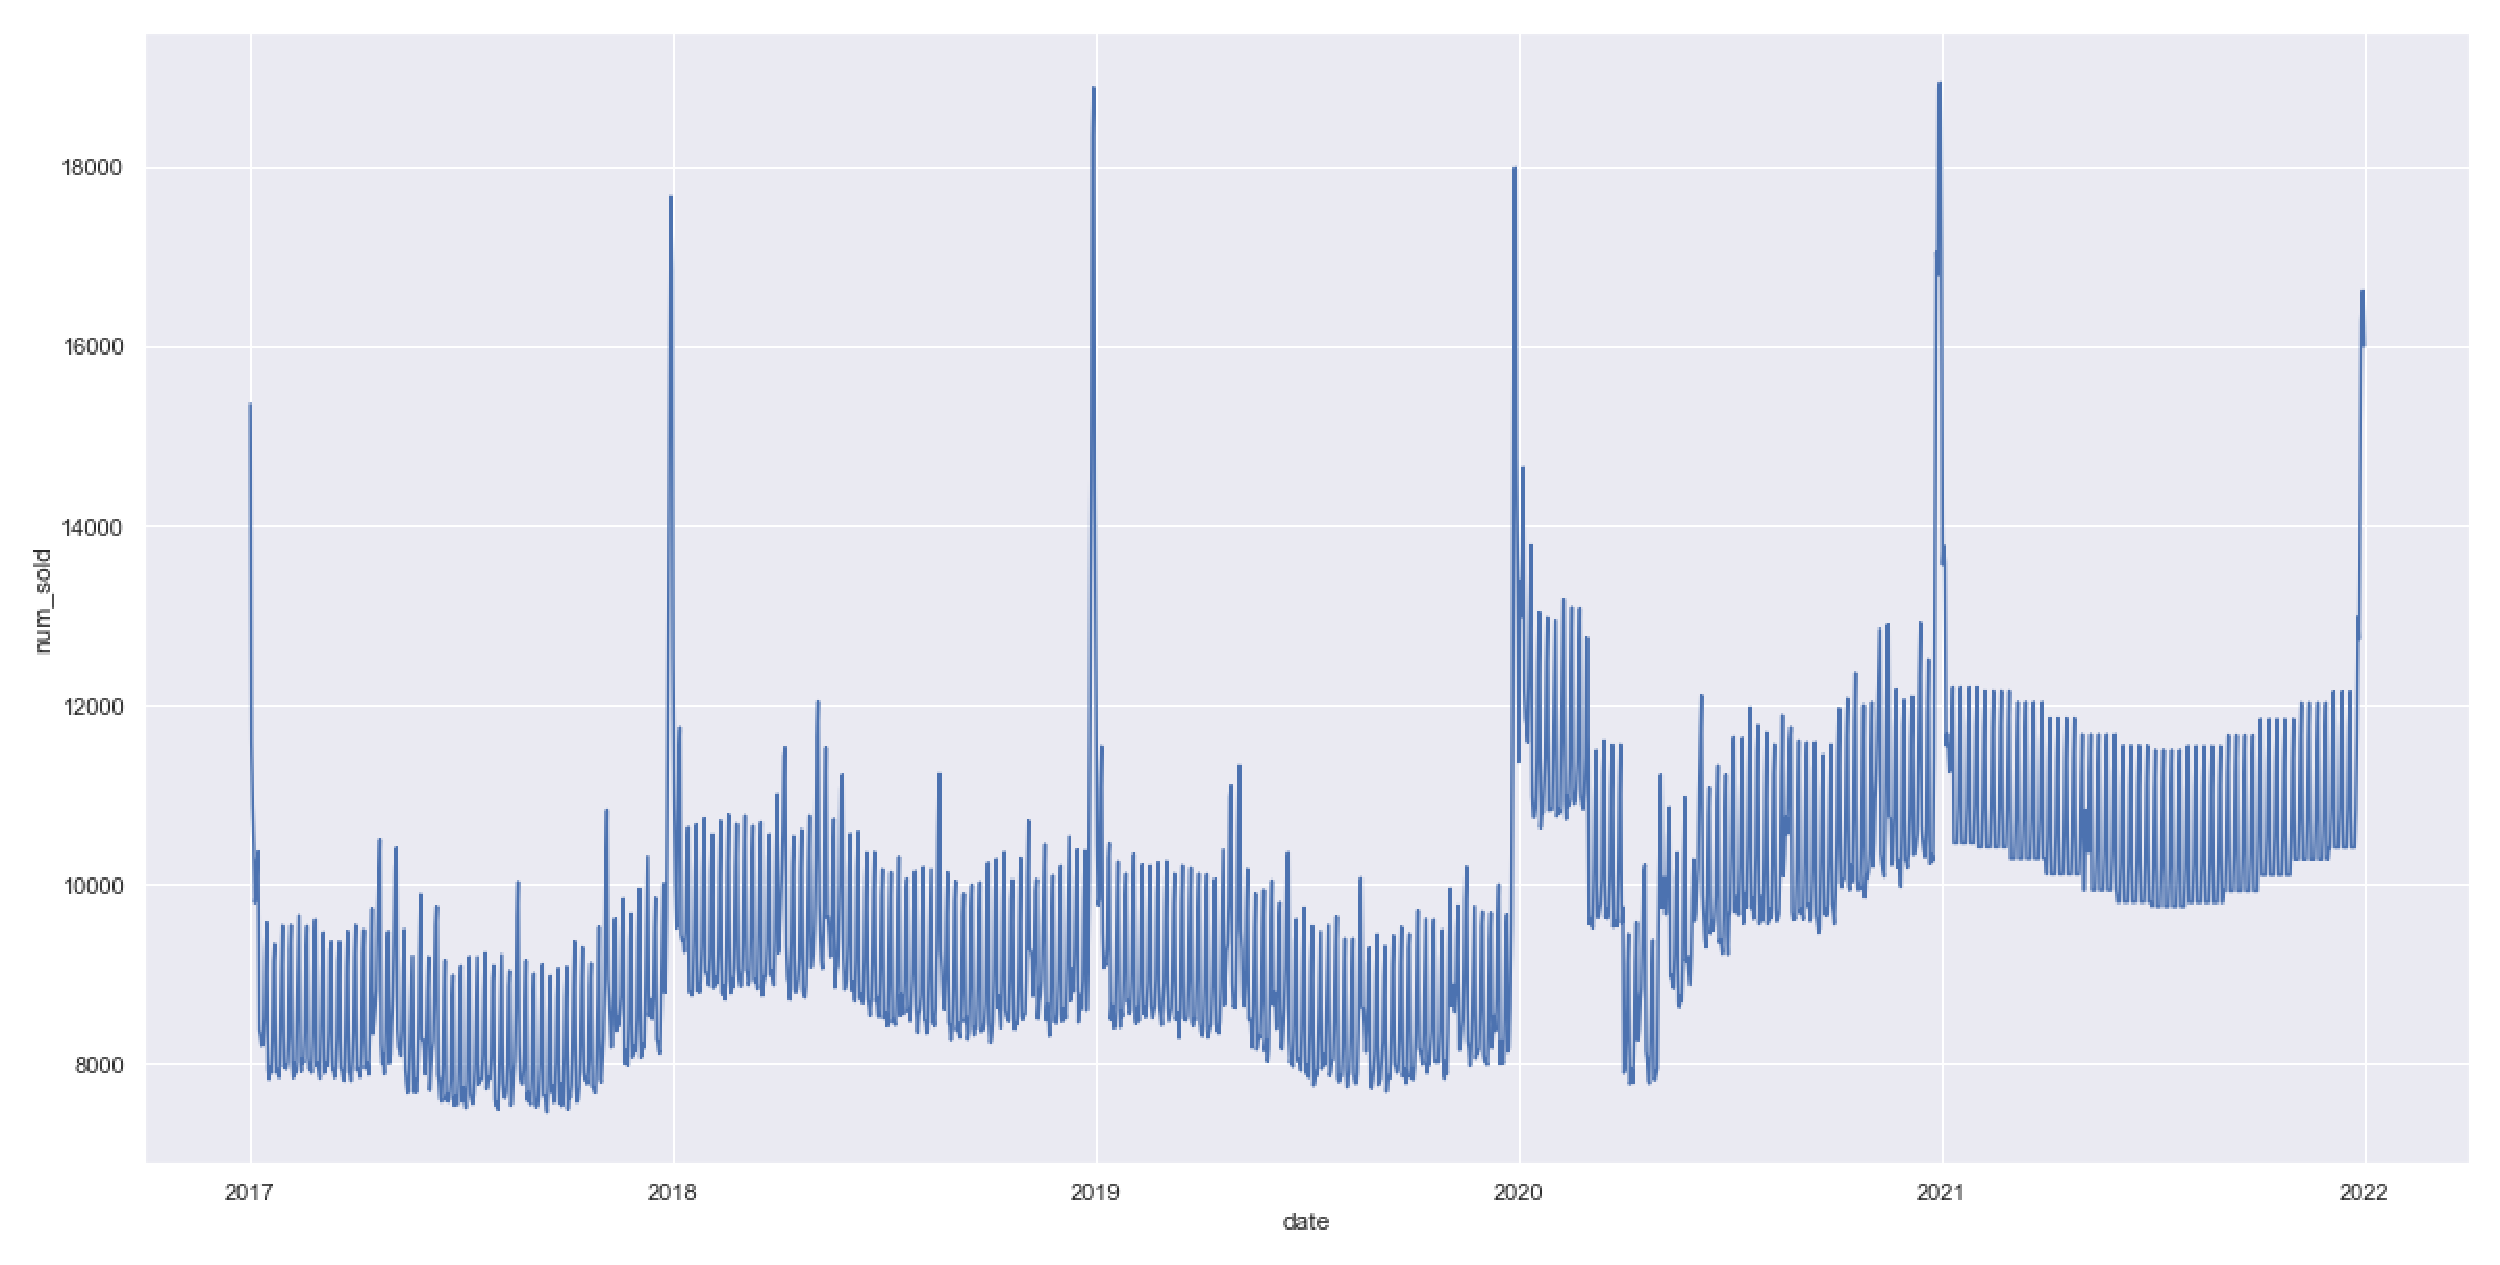
\includegraphics[scale=0.34]{total-sales.eps}
	%  \includegraphics[width=0.5\textwidth]{figures//OutAspect_target.eps}\\
	\caption{total sales forecasting}\label{fig:OutAspect-target}
\end{figure}

\end{slide}
%%
%%==========================================================================================


%%==========================================================================================
%%
\begin{slide}[toc=,bm=]{Product Ratio Forecast}

	We found that the proportion of sales for a product has a cyclical variation with a period of two years. Therefore, we assign the daily proportion of sales for each product in 2019 to 2021.
	\begin{figure}
		\centering
		\selectcolormodel{rgb}
		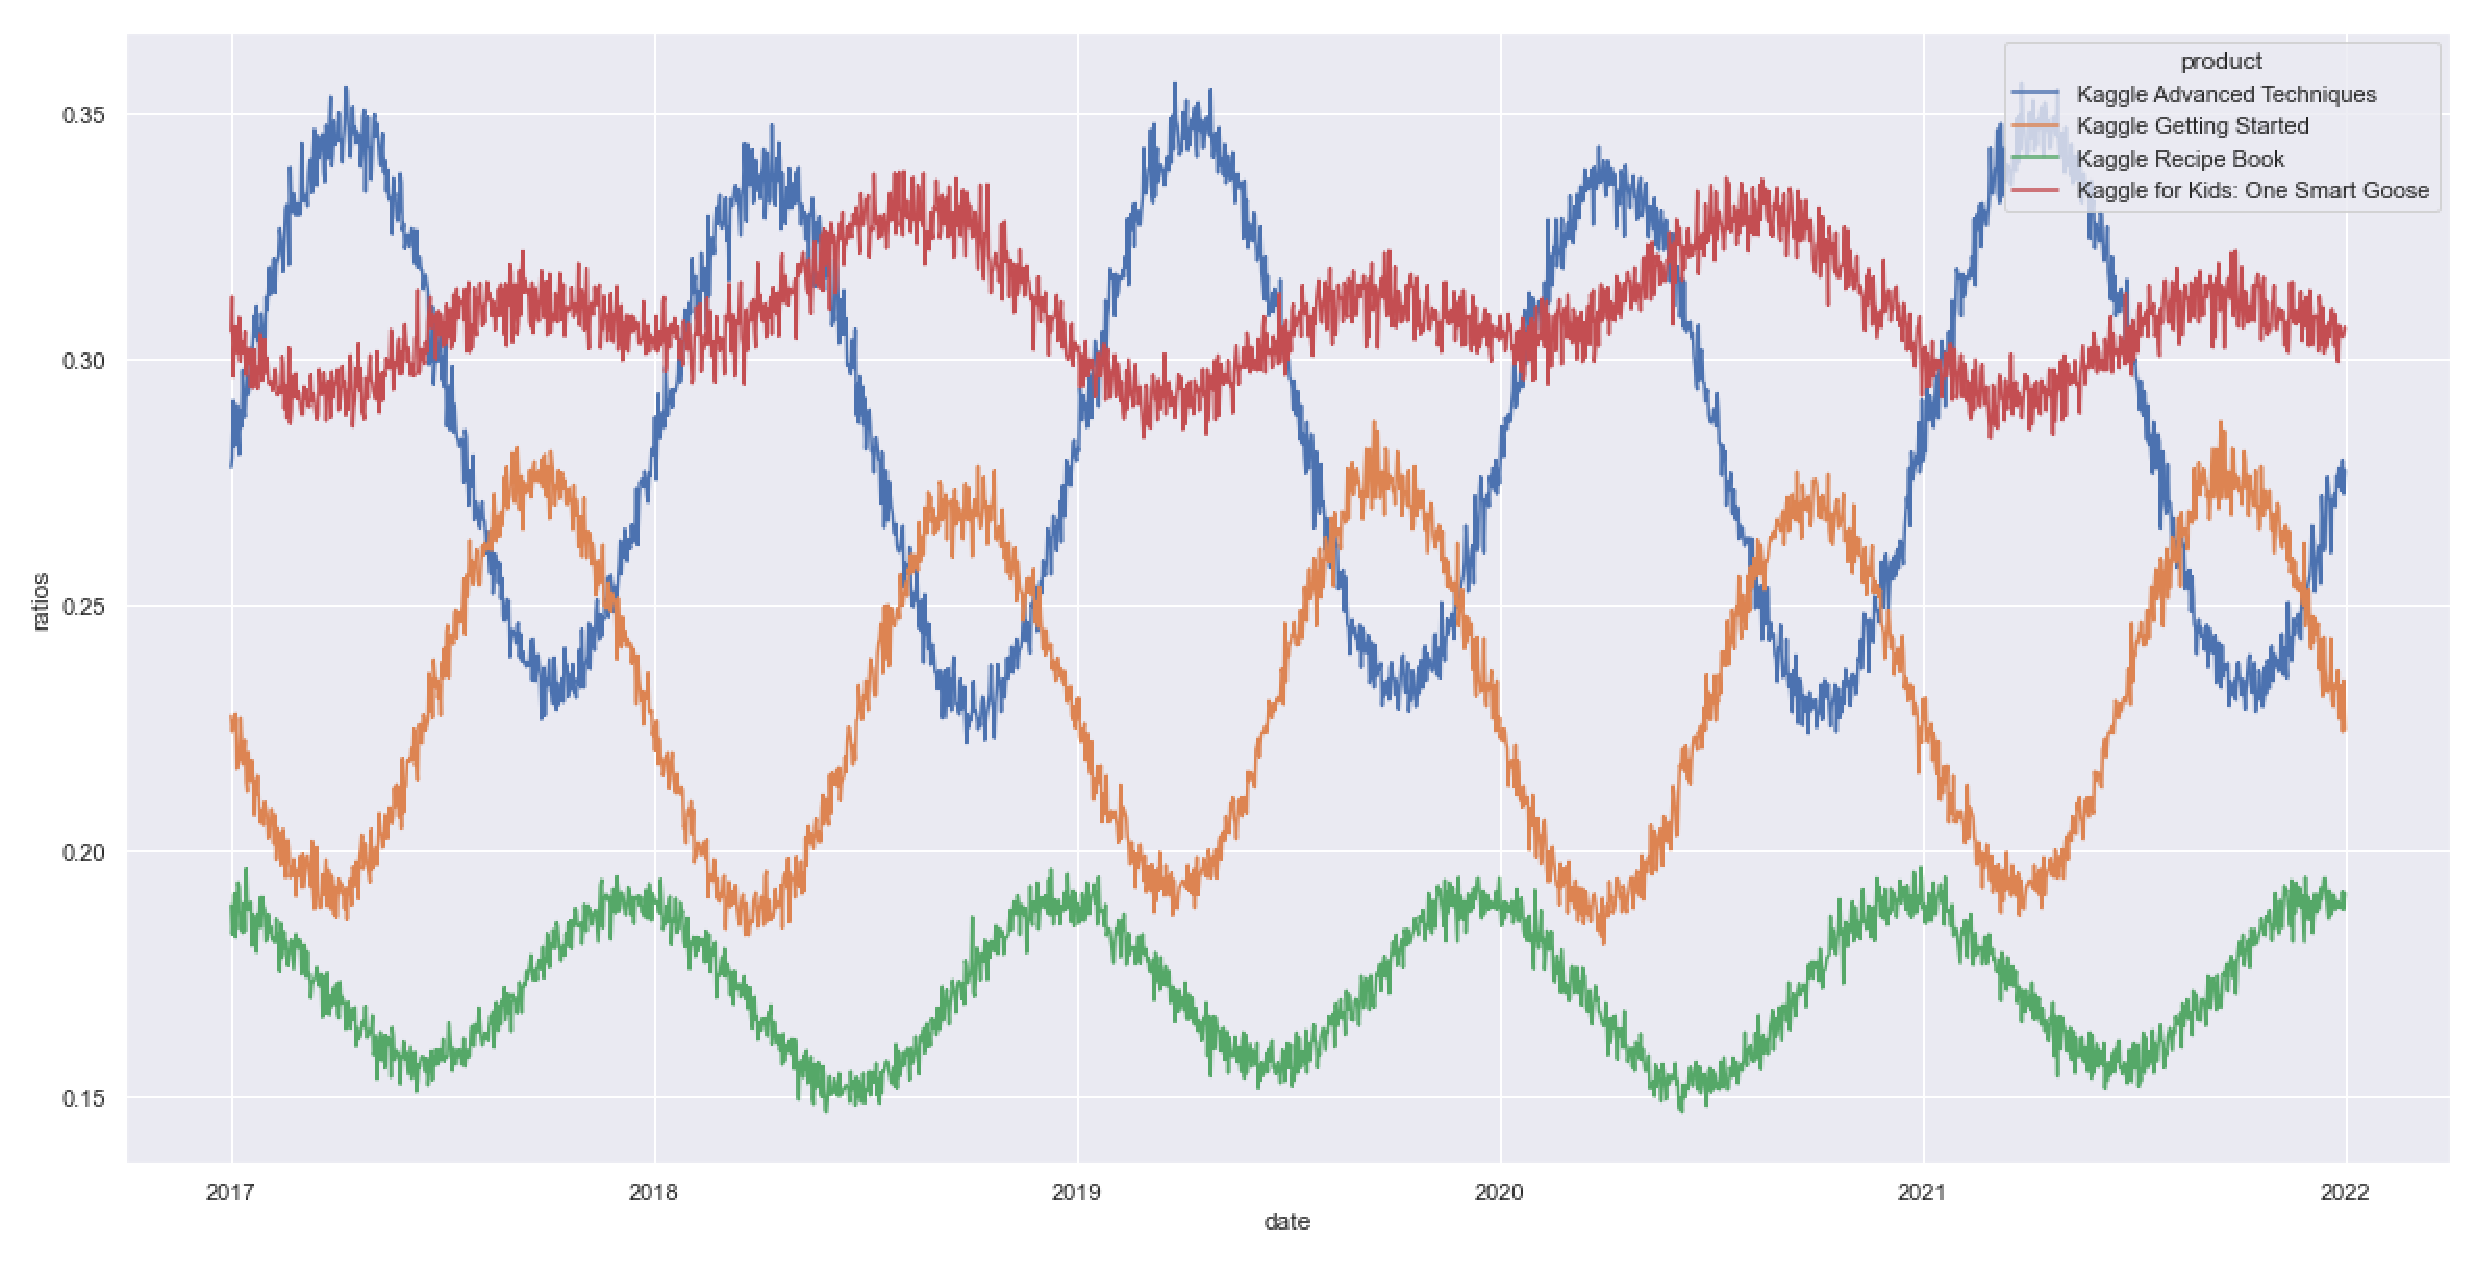
\includegraphics[scale=0.38]{product-ratio-for.eps}
		%  \includegraphics[width=0.5\textwidth]{figures//OutAspect_target.eps}\\
		\caption{Product Ratio Forecast}\label{fig:OutAspect-target}
	\end{figure}
	
\end{slide}
%%==========================================================================================
\begin{slide}[toc=,bm=]{Country and Store Ratio Forecast}
\begin{itemize}
	\item We assume that the proportion of sales in countries in 2021 is the same as in 2020. In 2020, the proportion of sales in countries accounts for \textcolor{red}{1/6},
	\item The proportion of different stores remains fixed, KaggleMart accounts for \textcolor{red}{75\%}, and KaggleRama accounts for \textcolor{red}{25\%}
\end{itemize}
	\begin{figure}
		\centering
		\selectcolormodel{rgb}
		\includegraphics[scale=0.2]{final-for.eps}
		%  \includegraphics[width=0.5\textwidth]{figures//OutAspect_target.eps}\\
		\caption{Final Forecasting}\label{fig:OutAspect-target}
	\end{figure}
	
\end{slide}

\section{Conclusion}

%%==========================================================================================
%%
\begin{slide}[toc=,bm=]{Conclusion}
\begin{itemize}
\item
\smallskip
This is a time series forecasting problem that includes complex elements.

\item
\smallskip
Simplifying the effects of complex factors through analyzing patterns discovered through single factor analysis.

\item
\smallskip
Use linear regression method to predict the relationship between sales volume and time characteristics.

\end{itemize}

%%==========================================================================================
%%==========================================================================================

\end{slide}
%%
%%==========================================================================================


%%==========================================================================================
%
\begin{slide}[toc=,bm=]{Questions?}
\begin{center}
\begin{figure}
    \animategraphics[autoplay, loop, height=0.4\textheight]{5}{./graphics//gif//question//q_}{1}{30}
\end{figure}
\end{center}
\end{slide}
%%
%%==========================================================================================


%%==========================================================================================
% TODO: Contact Page
\begin{wideslide}[toc=,bm=]{Contact Information}
\centering
\vspace{\stretch{1}}
\twocolumn[
lcolwidth=0.35\linewidth,
rcolwidth=0.65\linewidth
]
{
% \centerline{\includegraphics[scale=.2]{tulip-logo.eps}}
}
{
\vspace{\stretch{1}}
Jiahong Lin\\
School of Economics and Management\\
Nanjing University of Science and Technology, China
\begin{description}
 \item[\textcolor{orange}{\faEnvelope}] \href{mailto:kksmi18@163.com}
 {\textsc{\footnotesize{kksmi18@163.com}}}


\end{description}
}
\vspace{\stretch{1}}
\end{wideslide}

\end{document}

\endinput
